\documentclass[12pt]{article}

\usepackage{amsmath}
\usepackage{amssymb}
\usepackage[pdftex]{graphicx}
\usepackage{multicol}

\date{September 2021}
\title{Optimisation with Progressive Sharpening}
\author{Sahil Trivedi}

\begin{document}
	\maketitle
	
	\begin{multicols}{2}
		\section{Abstract}
		Introducing Progressive Sharpening, a method for optimising convolutional and fully connected layers in neural networks. This is achieved by creating incrementally denoised (blurred) copies of the training data. Training is initialised with the most denoised samples, and every few epochs we progressively sharpen the samples until the network converges on the orginal training data. We discuss the mathematical intuition of our technique and benchmark it against SoTA models on image recognition datasets. 
		
		\section{Introduction}
		Gradient descent optimises the weights of a network by minimising the error for it's neurons' activation values. A common tradeoff associated with gradient descent is it's tendency to converge training around local minima. Despite extensive research in the area of learning rate optimisation, avoiding local minima remains a recurring challenge in deep learning.
		\\\\
		During denoising, high level features are preserved while obscure features are smoothened out of the data. This is leveraged early on during training as we want the network paramters to distinguish high level features and avoid lower level features associated with local minima. As training progresses and high level features are generalised, we proceed to increase the level of detail in our training data making the network focus on more obscure features towards the end of training.
		\\\\
		It is well established that vision in human infants is blurred and improves it's focus as time passes. We discuss the mathematical working of progressive denoising in Section 6 of this paper.  
		
		\section{Denoising Training Samples}
		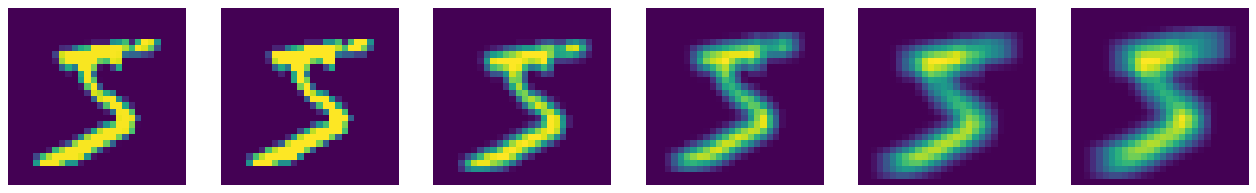
\includegraphics[width=\linewidth]{assets/denoise.png}
		\\\\
		The figure above illustrates an original sample on the extreme left followed by it's progressively denoised copies. The original image is from the MNIST dataset and the denoising is carried out using low pass filters. The kernels for these filters are represented by the following matrices:
		\\\\
		$$ kernel_{1} = \begin{bmatrix}
			1
		\end{bmatrix} / 1 $$
		$$ kernel_{2} = \begin{bmatrix}
			1 & 1 \\
			1 & 1
		\end{bmatrix} / 4$$
		$$ kernel_{3} = \begin{bmatrix}
			1 & 1 & 1 \\
			1 & 1 & 1 \\
			1 & 1 & 1
		\end{bmatrix} / 9$$
		$$ kernel_{4} = \begin{bmatrix}
			1 & 1 & 1 & 1 \\
			1 & 1 & 1 & 1 \\
			1 & 1 & 1 & 1 \\
			1 & 1 & 1 & 1
		\end{bmatrix} / 16$$
		$$ kernel_{5} = \begin{bmatrix}
			1 & 1 & 1 & 1 & 1 \\
			1 & 1 & 1 & 1 & 1 \\
			1 & 1 & 1 & 1 & 1 \\
			1 & 1 & 1 & 1 & 1 \\
			1 & 1 & 1 & 1 & 1
		\end{bmatrix} / 25$$
		\\\\
		Since $kernel_{1}$ denotes an identity transform, the first two images are identical and the latter four are progressively denoised. We apply the said convolutions to the training dataset which returns denoised copies of the training data. These copies are passed to the Convolutional Neural Network while training in a predetermined order.
		
		\section{Training}
		The multiple sets of training data obtained from the previous step can be referred to as $t_{1},t_{2},...t{5}$ where 
		$$t_{n} = training\_data \circledast kernel_{n} $$

			\subsection{Early Training}
			\subsection{Sharpening Training Samples}
			\subsection{Convergence on Original Samples}
			
		\section{Benchmarking}
		
		\section{Mathematical Explanation}
		Gradient descent optimises the weights of a network by minimising the error in it's neurons' activation values. A common tradeoff associated with gradient descent is it's tendency to converge training around local minima. Learning Rate Optimisation is generally employed to address this.
		\\
		- Visualising W vs E hypersurface
		
	\end{multicols}

	\begin{multicols}{2}
		
	\end{multicols}
	
	
	
	
	
\end{document}
